\section*{TEOREMA DI HUYGENS-STEINER (assi paralleli)}

\begin{figure}[H]
\centering
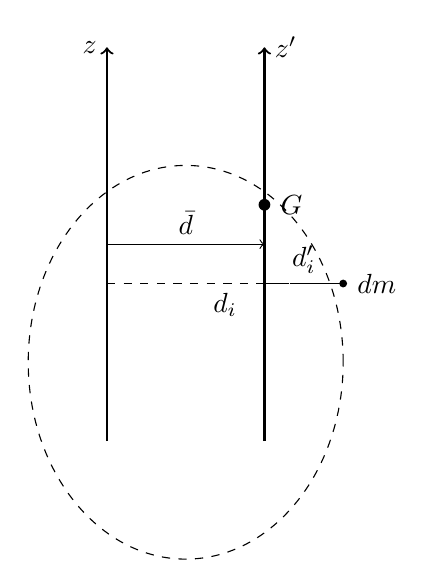
\begin{tikzpicture}
% Assi e corpo
\draw[thick, ->] (0, -2) -- (0, 3) node[left] {$z$};
\draw[thick, ->] (2, -2) -- (2, 3) node[right] {$z'$};
\draw (2, 1) node[circle, fill, inner sep=1.5pt, label=right:{$G$}] {};
\draw[dashed] (1, -1) ellipse (2cm and 2.5cm); % corpo rigido indicativo
\draw[->] (0, 0.5) -- (2, 0.5) node[midway, above] {$\bar{d}$};
\draw (3, 0) node[circle, fill, inner sep=1pt, label=right:{$dm$}] {};
\draw[dashed] (0, 0) -- (3, 0) node[midway, below] {$d_i$};
\draw[dashed] (2, 0) -- (3, 0) node[midway, above] {$d'_i$};
\end{tikzpicture}
\end{figure}

Il momento di inerzia di un corpo rigido rispetto ad un asse $z$ qualsiasi si calcola come:
$$ I_z = I_{z'} + M d^2 $$

Lo vediamo pk:
\begin{align*}
I_z &= \sum_i m_i d_i^2 = \sum_i m_i ( \bar{d_i'} + \bar{d} )^2 \\
&= \sum_i m_i ( {d'_i}^2 + d^2 + 2\bar{d} \cdot \bar{d'_i} ) \\
&= \underbrace{\sum_i m_i {d'_i}^2}_{= I_{z'}} + \underbrace{\sum_i m_i d^2}_{= M d^2} + \underbrace{2\bar{d} \cdot \sum_i m_i \bar{d'_i}}_{\substack{= 0 = x_G \\ \text{pk le coordinate} \\ \text{di } x_G \text{ nel CM } = 0}}
\end{align*}

$G \equiv CM$
\begin{equation}
I_z = I_{z'} + M d^2
\end{equation}

Quindi si deve conoscere $I_z$ e $I_{z'}$. Inoltre, dati infiniti assi equidistanti da $z'$, questi avranno lo stesso momento di inerzia; Dato invece un fascio di assi, quello che passa per il CM sarà quello che ha il momento di inerzia minore, poiché $d = 0$.

\subsection*{a) rotazione (intorno ad un asse FISSO)}
\begin{figure}[H]
\centering
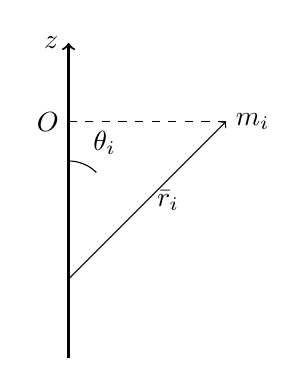
\begin{tikzpicture}
\draw[thick, ->] (0, -1) -- (0, 3) node[left] {$z$};
\draw[->] (0,0) -- (2,2) node[right] {$m_i$};
\draw[dashed] (0,2) -- (2,2);
\draw (1, 1) node[right] {$\bar{r}_i$};
\draw (0, 2) node[left] {$O$};
\draw (0, 1.5) arc (90:45:0.5) node[midway, above right] {$\theta_i$};
\end{tikzpicture}
\end{figure}
$d_i = r_i \cdot \sin \theta_i$ \quad $\bar{\omega} \parallel \hat{z}$

\begin{align*}
K &= \sum_i \frac{1}{2} m_i \bar{v}_i^2 = \frac{1}{2} \sum_i m_i ( \bar{\omega} \times \bar{r}_i )^2 \\
&= \frac{1}{2} \sum_i m_i ( \omega \cdot r_i \cdot \sin \theta_i )^2 \\
&= \frac{1}{2} \omega^2 \sum_i m_i ( r_i \sin \theta_i )^2 = \frac{\omega^2}{2} \sum_i m_i d_i^2 \\
&= \frac{1}{2} I_z \omega^2 = \frac{L_z^2}{2 I_z}
\end{align*}

\subsection*{b) rototraslazione}
In questo caso si sfrutta Koenig
\begin{align*}
K &= \frac{1}{2} M \bar{v}_{CM}^2 + K_{rel} = \frac{1}{2} M v_{CM}^2 + \sum_i m_i \frac{\bar{v}_i'^2}{2} = \frac{1}{2} M v_{CM}^2 + \frac{1}{2} \sum_i m_i ( \bar{\omega} \times \bar{r}_i' )^2 \\
&= \frac{1}{2} M v_{CM}^2 + \frac{1}{2} I_{CM} \omega^2 \\
&= K_{TRASL} + K_{ROTAZ}
\end{align*}

\subsection*{c) rotolamento}
\begin{figure}[H]
\centering
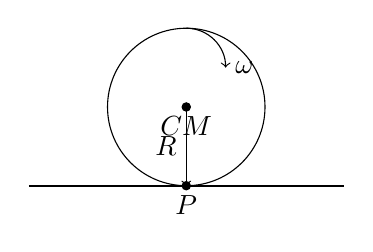
\begin{tikzpicture}
\draw[thick] (-2, 0) -- (2, 0);
\draw (0, 1) circle (1cm);
\draw[fill] (0, 1) circle (1.5pt) node[below] {$CM$};
\draw[->] (0, 1) -- (0, 0) node[midway, left] {$R$};
\draw[fill] (0, 0) circle (1.5pt) node[below] {$P$};
\draw[->] (0, 2) arc (90:0:0.5) node[right] {$\omega$};
\end{tikzpicture}
\end{figure}

$v_P = 0$ \quad $v_{CM} = \omega R$

\begin{align*}
K &= K_{CM} + K_{rel} = \frac{M}{2} v_{CM}^2 + \frac{\omega^2}{2} I_{CM} \\
&= \frac{M}{2} \omega^2 R^2 + \frac{I_{CM}}{2} \omega^2 = \frac{\omega^2}{2} ( I_{CM} + M R^2 ) \\
&= \frac{\omega^2}{2} I_P
\end{align*}

L'eventuale inclinazione del piano non cambia il rotolamento ($v_{CM} = \omega r$, $a_{CM} = \alpha r$).
- rotazione su CM + traslazione di CM ($v_{CM} = \omega R$)
- rotazione istantanea su P ($v_P = 0$)
